\begin{figure}[h]
    \centering
    \begin{subfigure}[b]{0.4\textwidth}
        \centering
        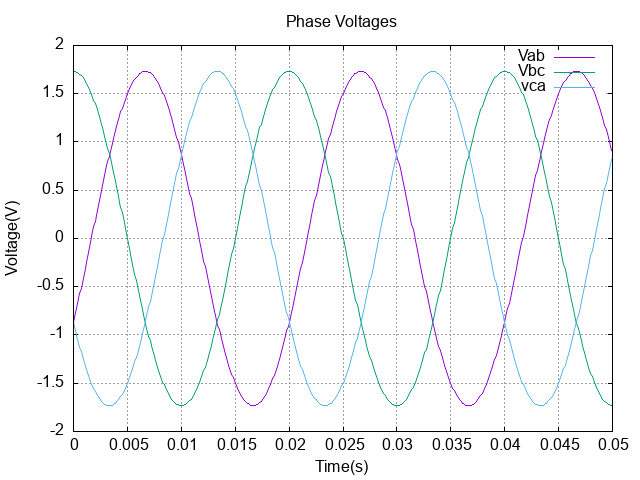
\includegraphics[width=\textwidth]{Phase_Voltages.png}
        \caption{Phase Voltages}
        \label{fig:Phase Voltages}
    \end{subfigure}
    \begin{tikzpicture}
        \node at (0,0) {};
        \draw[->, thick] (0,2.5) -- (1,2.5);
    \end{tikzpicture}
    \begin{subfigure}[b]{0.4\textwidth}
        \centering
        \includegraphics[width=\textwidth]{Line_Voltages.png}
        \caption{Line Voltages}
        \label{fig:Line Voltages}
    \end{subfigure}
\end{figure}

\subsection{Why Measure Phase Voltage?}
In three-phase electrical systems, the measurement of phase voltages becomes
critical due to the unavailability of the neutral point. This unavailability
means that direct measurement of line voltages is not feasible. Phase voltage
refers to the voltage measured across a single component within the three-phase
system, typically between a phase (live) wire and the neutral point. These
measurements are essential because they are the only voltages directly
accessible within the system. Despite this, most voltage transformations and
analyses are conventionally performed on line voltages, which represent the
voltage difference between any two phases in the system. To bridge this gap, it
is imperative to convert the measured phase voltages to line voltages using
precise voltage transformations.

\subsection{Need for Conversion from Phase to Line Voltage}
In a three-phase system, the primary objective is to regulate both the line
current and line voltage accurately. Line voltages, which are the voltages
between any two phases, are crucial for determining the overall performance and
stability of the system. However, since we are limited to measuring phase
voltages, a reliable conversion mechanism is necessary to translate these
measurements into line voltages. This conversion is essential for achieving
accurate control and analysis of the system's electrical parameters. By
converting phase voltages to line voltages, we can apply standard voltage
transformation techniques and ensure that the control strategies and safety
mechanisms are based on accurate and relevant data.

\subsection{Why Simply Dividing by the Square Root of 3 is Insufficient}
A common misconception is that dividing the measured phase voltage by the
square root of 3 will yield the correct line voltage. This approach is based on
the RMS (Root Mean Square) values and is only accurate for calculating the
magnitude of the line voltage under steady-state, balanced conditions. The
relationship \(phase\ voltage = \sqrt{3} \times line\ voltage\) holds true only
for the RMS values of sinusoidal voltages in a perfectly balanced system.
However, for dynamic applications, such as those involving digital signal
processing (DSP), we require instantaneous line voltages rather than just RMS
magnitudes.\\

Instantaneous voltages account for the real-time variations and phase
differences that occur in practical systems. Therefore, a more robust method is
necessary to obtain these instantaneous values accurately. To address this
requirement, we use a transformation matrix that accurately converts the phase
voltages to line voltages. The transformation matrix employed is:

\begin{equation*}
    T_{line} =
    \begin{bmatrix}
        \frac{2}{3}  & \frac{1}{3}  & 0 \\
        \frac{-1}{3} & \frac{1}{3}  & 0 \\
        \frac{-1}{3} & \frac{-2}{3} & 0
    \end{bmatrix}
\end{equation*}

This matrix provides a precise method to convert the three measured phase
voltages into their corresponding line voltages, ensuring that the
instantaneous values required for DSP and other real-time control applications
are accurately obtained. This approach eliminates the inaccuracies associated
with simple RMS-based conversion and allows for a more accurate representation
of the system's electrical characteristics in real-time operations.

\subsection{Derivation of the Transformations}
For this conversion, we need to define a matrix, so let's look at the
derivation for such a matrix.

Let \( V_a, V_b, V_c \) be the phase voltages given by:
\[
    V_a = \sin(\omega t)
\]
\[
    V_b = \sin(\omega t - 120^\circ)
\]
\[
    V_c = \sin(\omega t + 120^\circ)
\]

The line voltages \( V_{ab}, V_{bc}, V_{ca} \) are given by:
\[
    V_{ab} = V_a - V_b
\]
\[
    V_{bc} = V_b - V_c
\]
\[
    V_{ca} = V_c - V_a
\]

Also, we know that:
\[
    V_a + V_b + V_c = 0
\]

Let us assume two matrices: \( P \), representing phase voltages, and \( L \),
representing line voltages:
\[
    P = \begin{bmatrix}
        V_a \\
        V_b \\
        V_c \\
    \end{bmatrix}
\]
\[
    L = \begin{bmatrix}
        V_{ab} \\
        V_{bc} \\
        V_{ca} \\
    \end{bmatrix}
\]

Let \( T \) be a transformation matrix from \( P \) to \( L \):
\[
    L = T \cdot P
\]

We can define \( T \) as:
\[
    T = \begin{bmatrix}
        1  & -1 & 0  \\
        0  & 1  & -1 \\
        -1 & 0  & 1  \\
    \end{bmatrix}
\]

Since the inverse of \( T \) does not exist, we redefine it as:
\[
    \begin{bmatrix}
        V_{ab} \\
        V_{bc} \\
        V_{ca} \\
        0      \\
    \end{bmatrix} = \begin{bmatrix}
        1  & -1 & 0  & 1 \\
        0  & 1  & -1 & 1 \\
        -1 & 0  & 1  & 1 \\
        1  & 1  & 1  & 1 \\
    \end{bmatrix} \begin{bmatrix}
        V_a \\
        V_b \\
        V_c \\
        0   \\
    \end{bmatrix}
\]

Taking the inverse of \( T \):
\[
    T^{-1} = \begin{bmatrix}
        \frac{2}{9}  & -\frac{1}{9} & -\frac{4}{9} & \frac{1}{3} \\
        -\frac{4}{9} & \frac{2}{9}  & -\frac{1}{9} & \frac{1}{3} \\
        -\frac{1}{9} & -\frac{4}{9} & \frac{2}{9}  & \frac{1}{3} \\
        \frac{1}{3}  & \frac{1}{3}  & \frac{1}{3}  & 0           \\
    \end{bmatrix}
\]

Solving the matrix:
\[
    V_a = \frac{2}{9}V_{ab} - \frac{1}{9}V_{bc} - \frac{4}{9}V_{ca}
\]
\[
    V_b = -\frac{4}{9}V_{ab} + \frac{2}{9}V_{bc} - \frac{1}{9}V_{ca}
\]
\[
    V_c = -\frac{1}{9}V_{ab} - \frac{4}{9}V_{bc} + \frac{2}{9}V_{ca}
\]

We also know that \( V_{ab} + V_{bc} + V_{ca} = 0 \), so:
\[
    V_{ca} = -V_{ab} - V_{bc}
\]

Thus:
\[
    V_a = \frac{2}{3}V_{ab} + \frac{1}{3}V_{bc}
\]
\[
    V_b = -\frac{1}{3}V_{ab} + \frac{1}{3}V_{bc}
\]
\[
    V_c = -\frac{1}{3}V_{ab} - \frac{2}{3}V_{bc}
\]

So, we can define the transformation matrix as:
\[
    T_{line}^{-1} = \begin{bmatrix}
        \frac{2}{9}  & -\frac{1}{9} & -\frac{4}{9} \\
        -\frac{4}{9} & \frac{2}{9}  & -\frac{1}{9} \\
        -\frac{1}{9} & -\frac{4}{9} & \frac{2}{9}  \\
    \end{bmatrix}
\]
